% VUT FIT MITAI
% PDS 2021/2022
% Project: Identification of Mobile Traffic using TLS Fingerprinting
% Author: Vladimir Dusek
% Login: xdusek27

%%%%%%%%%%%%%%%%%%%%%%%%%%%%%%%%%%%%%%%%%%%%%%%%%%%%%%%%%%%%%%%%%%%%%%%%%%%%%%%%

\documentclass[12pt,a4paper]{article}

\usepackage[english,czech]{babel}
\usepackage[utf8]{inputenc}
\usepackage[T1]{fontenc}
\usepackage{geometry}
\usepackage{listings}
\usepackage{amsmath}
\usepackage{amssymb}
\usepackage[justification=centering]{caption}
\usepackage{subcaption}
\usepackage{graphicx}
\usepackage[ruled,vlined,linesnumbered]{algorithm2e}
\usepackage{float}
\usepackage{xcolor}
\usepackage{csquotes}
\usepackage[bottom]{footmisc}
\usepackage[nottoc,numbib]{tocbibind}
\usepackage{hhline}

\newtheorem{theorem}{Theorem}

\makeatletter
\renewcommand*\env@matrix[1][*\c@MaxMatrixCols c]{%
    \hskip -\arraycolsep
    \let\@ifnextchar\new@ifnextchar
    \array{#1}}
\makeatother

\MakeOuterQuote{"}

\PassOptionsToPackage{hyphens}{url}\usepackage[hidelinks,unicode]{hyperref}

% Page dimensions
\geometry
{
    top = 3cm,
    bottom = 3cm,
    left = 3cm,
    right = 3cm
    % text = {17cm, 24cm}
}

% Path for figures
\graphicspath{{figures/}}

% Colors for listings
\definecolor{codegreen}{rgb}{0,0.6,0}
\definecolor{codegray}{rgb}{0.5,0.5,0.5}
\definecolor{codepurple}{rgb}{0.58,0,0.82}
\definecolor{backcolour}{rgb}{0.95,0.95,0.92}

\lstdefinelanguage{myLang} {
    % list of keywords
    morekeywords={
        import,
        if,
        while,
        for,
        then,
        else,
        do
    },
    sensitive=false, % keywords are not case-sensitive
    morecomment=[l]{//}, % l is for line comment
    morecomment=[s]{/*}{*/}, % s is for start and end delimiter
    morestring=[b]" % defines that strings are enclosed in double quotes
}

% Style for listings
\lstdefinestyle{mystyle}{
    language={myLang},
    backgroundcolor=\color{backcolour},
    commentstyle=\color{codegreen},
    keywordstyle=\color{magenta},
    numberstyle=\tiny\color{codegray},
    stringstyle=\color{codepurple},
    basicstyle=\ttfamily\footnotesize,
    breakatwhitespace=false,
    breaklines=true,
    captionpos=t,
    keepspaces=true,
    % numbers=left,
    numbersep=5pt,
    showspaces=false,
    showstringspaces=false,
    showtabs=false,
    tabsize=4
}
\lstset{style=mystyle}

%%%%%%%%%%%%%%%%%%%%%%%%%%%%%%%%%%%%%%%%%%%%%%%%%%%%%%%%%%%%%%%%%%%%%%%%%%%%%%%%

\begin{document}

\begin{titlepage}
    \begin{center}

        % {\Huge\textsc{Vysoké učení technické v~Brně}} \\
        % \bigskip
        % {\huge\textsc{Fakulta informačních technologií}} \\

        \begin{figure}[htb]
            \centering
            
\includegraphics[width=0.85\hsize]{fitlogo.pdf}
        \end{figure}

        \vspace{\stretch{0.382}}

        {\Huge Identifikace mobilního síťového provozu} \\
        \bigskip
        {\Huge pomocí TLS otisků} \\
        \bigskip
        \bigskip
        {\LARGE Přenos dat, počítačové sítě a protokoly (PDS)   }

        \vspace{\stretch{0.618}}
    \end{center}

    {\Large \today \hfill Vladimír Dušek, xdusek27}

\end{titlepage}

% \begin{center}
%     {\Huge Game Theory (THE)} \\ [1.25em]
%     {\huge Brno University of Technology} \\ [1.25em]
%     {\huge Strategie sobeckého těžení v~Bitcoinu} \\ [1.6em]
%     {\Large \textit{Dušek Vladimír - xdusek27@stud.fit.vutbr.cz}} \\ [0.7em]
%     {\Large \textit{\today}}
%  \end{center}

%%%%%%%%%%%%%%%%%%%%%%%%%%%%%%%%%%%%%%%%%%%%%%%%%%%%%%%%%%%%%%%%%%%%%%%%%%%%%%%%

\tableofcontents
\newpage

%%%%%%%%%%%%%%%%%%%%%%%%%%%%%%%%%%%%%%%%%%%%%%%%%%%%%%%%%%%%%%%%%%%%%%%%%%%%%%%%

%%%%%%%%%%%%%%%%%%%%%%%%%%%%%%%%%%%%%%%%%%%%%%%%%%%%%%%%%%%%%%%%%%%%%%%%%%%%%%%%

\section{Bitcoin jako decentralizovaný finanční systém}
\label{sec_bitcoin}

Klíčovým bodem fungování Bitcoinu je veřejná distribuovaná "účetní kniha", zvaná \textit{blockchain}. V~té jsou zaznamenány všechny transakce, které kdy byly v~bitcoinové síti uskutečněny. Každý uzel disponuje svojí vlastní kopií, kterou si aktualizuje. Velmi zjednodušeně jsou transakce zapisovány následovně: z~adresy $X$ je odesláno $N$ bitcoinů na adresu $Y$. Uživatel disponuje typicky mnoha adresami, v~ideálním případě novou adresou pro každou platbu.

%%%%%%%%%%%%%%%%%%%%%%%%%%%%%%%%%%%%%%%%%%%%%%%%%%%%%%%%%%%%%%%%%%%%%%%%%%%%%%%%

\subsection{Autentizace}
\label{sec_bitcoin_autentizace}

V~systému je bezpochyby nutné autentizovat vlastníky jednotlivých mincí. To je zajištěno pomocí asymetrické kryptografie. Jednotlivé mince uživatelů jsou přiřazeny k~pseudonymům -- bitcoinovým adresám. Adresa je pouze derivátem veřejného klíče. Výhradně ten, kdo disponuje soukromým klíčem, který náleží danému veřejnému klíči, může vygenerovat validní digitální podpis. Tím se v~síti autentizuje jako vlastník mince na dané adrese a může vytvořit platnou transakci.

Protokol je navržen tak, aby každý uživatel mohl disponovat unikátní adresou pro každou svoji minci. Klíče k~jednotlivým adresám uživatelé mají uložené ve svých peněženkách. Peněženka je software pro správu klíčů a vytváření transakcí. Vytvořená transakce je zaslána konkrétnímu bitcoinovému uzlu, který, je-li transakce validní, ji zašle dalším uzlům.

%%%%%%%%%%%%%%%%%%%%%%%%%%%%%%%%%%%%%%%%%%%%%%%%%%%%%%%%%%%%%%%%%%%%%%%%%%%%%%%%

\subsection{Opětovné utracení}
\label{sec_bitcoin_opetovne_utraceni}

Opětovné utracení (\textit{replay attack}) znamená, že uživatel svoji konkrétní minci utratí vícekrát. Nic uživateli nebrání, vytvořit transakci s~validním podpisem, který utrácí minci, kterou již někdy dřívě utratil. V~systému je nutné rozpoznávat, které mince již byly utraceny a které nikoliv.

V~bitcoinovém protokolu je toto řešeno sledováním historie mincí. Jednotlivé mince řetězíme za sebe, tak jak v~jednotlivých transakcích putují napříč různými adresami. Známe tedy historii všech mincí od jejich vzniku (viz sekce~\ref{sec_bitcoin_tezeni}) až po jejich současnost -- tzv. neutracený transakční výstup (UTXO -- \textit{Unspent transaction output}). Výhradně UTXO může figurovat jako vstup transakce, tím je zajištěno, že vlastník nemůže stejnou "minci" utratit vícekrát.

\begin{figure}[ht]
    \centering
    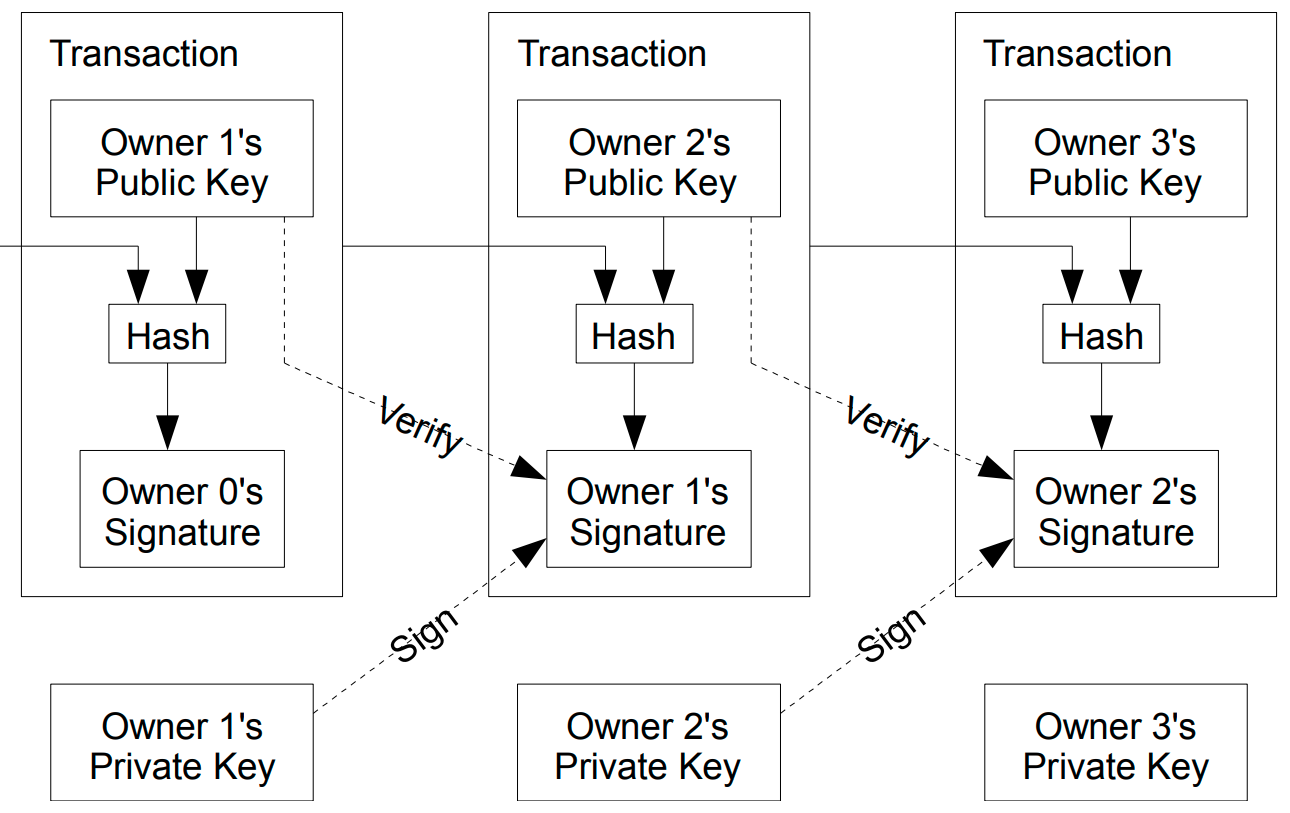
\includegraphics[width=0.75\linewidth]{transaction.png}
    \caption{Bitcoinové transakce~\cite{bib_white_paper}.}
    \label{fig_transaction}
\end{figure}

%%%%%%%%%%%%%%%%%%%%%%%%%%%%%%%%%%%%%%%%%%%%%%%%%%%%%%%%%%%%%%%%%%%%%%%%%%%%%%%%

\subsection{Dvojí utracení}
\label{sec_bitcoin_dvoji_utraceni}

Dvojí utracení (\textit{double spend attack}) je takový problém, kdy uživatel disponující UTXO $X$, vytvoří transakci, ve které utrácí UTXO $X$ na adresu $Y$ a zároveň jinou transakci, ve které utrácí UTXO $X$ na adresu $Z$. Každou transakci pošle jinému uzlu. Ten transakci zvaliduje a pošle dále do sítě. Jelikož jsme si doposud nepředstavili žádný systém časových razítek, síť není schopná vyhodnotit, která transakce je platná (byla zadána jako první) a která je neplatná (má jako vstup již utracené UTXO).

Ochrana před dvojím utracením je řešena právě \textit{blockchainem}. Transakce jsou agregovány do bloků, které jsou zhruba každých 10 minut uzavírány. Každý blok obsahuje kromě samotných transakcí také hash (SHA-256) předchozího bloku. Tím jsou bloky zřetězeny za sebe (odtud název blockchain) a vzniká chronologické uspořádání. Pokud by někdo chtěl měnit informace v~již uzavřeném bloku (blok nad kterým staví již další blok), musí přepočítat hashe všech následujících bloků\footnote{Z tohoto hlediska funguje podobným způsobem verzovací distribuovaný systém Git.}.

%%%%%%%%%%%%%%%%%%%%%%%%%%%%%%%%%%%%%%%%%%%%%%%%%%%%%%%%%%%%%%%%%%%%%%%%%%%%%%%%

\subsection{Důkaz prací}
\label{sec_bitcoin_dukaz_praci}

V~bitcoinovém protokolu je konsenzus nastaven tak, že nejdelší blockchain je pravda. V~tuto chvíli by však bylo možné změnit jakoukoliv již zapsanou transakci, přepočítat hashe všech následujících bloků a prohlásit tuto verzi blockchainu za nejdelší řetězec a tím pádem pravdu.

Abychom tomuto zamezili, musí být zápis do blockchainu nákladná operace. Toho je v~Bitcoinu docíleno tak, že na hash bloku jsou kladeny nějaké nároky. Konkrétně takové, že výsledný hash musí být malé číslo. K~tomuto účelu je v~bloku místo pro náhodné číslo, tzv. \textit{nonce}. Pokud chce někdo přidat nový blok do blockchainu, musí najít takové číslo, které způsobí, že výsledný hash bloku bude odpovídat současným nárokům sítě. Tyto nároky se v~průběhu času mění podle výpočetního výkonu celé sítě tak, aby bloky byly uzavírány v~průměru každých 10 minut.

Tento koncept se nazývá důkaz prací (z~anglického \textit{proof of work}).

\begin{figure}[ht]
    \centering
    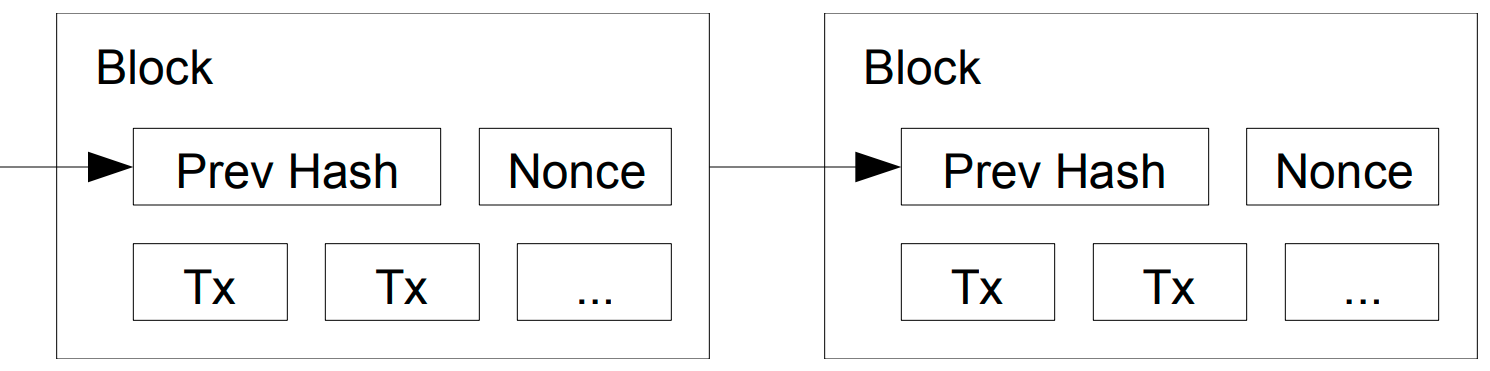
\includegraphics[width=0.75\linewidth]{blockchain.png}
    \caption{Chronologické zřetězení bloků za sebe -- \textit{blockchain}~\cite{bib_white_paper}.}
    \label{fig_blockchain}
\end{figure}

%%%%%%%%%%%%%%%%%%%%%%%%%%%%%%%%%%%%%%%%%%%%%%%%%%%%%%%%%%%%%%%%%%%%%%%%%%%%%%%%

\subsection{Těžení}
\label{sec_bitcoin_tezeni}

Proces hledání správných \textit{nonce} a zapisování nových bloků do blockchainu se nazývá těžení (\textit{Bitcoin Mining}). Entity, které tuto činnost vykonávají se nazývají těžaři (\textit{Bitcoin Miners}). Bitcoinový protokol motivuje uživatele tuto činnost provádět tak, že za uzavření bloku poskytuje odměnu v~podobě nově vzniklých bitcoinů. Ty jsou vytvořeny v~rámci tzv. \textit{coinbase} transakce, což je vždy první transakce v~bloku.

Těžař poskládá transakce dalších uživatelů do bloku, přidá hash předcházejícího bloku a generuje náhodná čísla jako potenciální \textit{nonce}. Z~toho pomocí hashovací funkce SHA-256 spočítá hash a zkontroluje, zda náhodou výsledný hash není dostatečně malé číslo. Pokud měl štěstí a je, blok je vytěžen a těžař ho rozpošle dalším uživatelům. Ti ho přijmou a začnou těžit další bloky nad ním.

Aby těžaři získávali odměnu v~pravidelných a více predikovatelných intervalech, začaly se formovat tzv. \textbf{těžařské pooly} (\textit{Mining Pool}). Několik těžařů spojí svůj výpočetní výkon a figurují jako jedna entita. Pokud některý z~nich vytěží blok, odměnu si rozdělí s~ostatními proporciálně dle jejich výpočetního výkonu.

Odměna za vytěžený blok se skládá ze dvou složek. Kromě již zmíněné \textit{coinbase} transakce s~nově vzniklými bitcoiny, dostane těžař také transakční odměny ze všech transakcí v~bloku. Uživatelé, chtějí-li motivovat těžaře, aby zahrnuli jejich transakci do bloku, platí transakční poplatky. Ty jsou definovány jako rozdíl mezi transakčními vstupy a transakčními výstupy, viz rovnice~\ref{eq_tx_fees}.

\begin{equation}
    in_1 + \ldots + in_n - out_1 - \ldots - out_m = tx\_fee
    \label{eq_tx_fees}
\end{equation}

%%%%%%%%%%%%%%%%%%%%%%%%%%%%%%%%%%%%%%%%%%%%%%%%%%%%%%%%%%%%%%%%%%%%%%%%%%%%%%%%

\newpage

%%%%%%%%%%%%%%%%%%%%%%%%%%%%%%%%%%%%%%%%%%%%%%%%%%%%%%%%%%%%%%%%%%%%%%%%%%%%%%%%

\section{Analýza problému}
\label{sec_problem_analysis}

Použitá technika rozpoznávání aplikací v~šifrovaném TLS provozu využívá tzv. JA3 otisky (\textit{fingerprints}). Ty byly představeny pány John B. Althouse, Jeff Atkinson a Josh Atkins v~roce 2015.\footnote{\url{https://github.com/salesforce/ja3}} Technika spočívá v~tom, že ze síťové komunikace jsou vyfiltrovány TLS \textit{handshake} packety. Z~packetů \textit{Client Hello} a \textit{Server Hello} jsou vyextrahovány následující položky: \textit{Handshake Version}, \textit{Cipher Suites}, \textit{Extensions}, \textit{Supported Groups} a \textit{Elliptic Curve Point Format}. Z~těchto informací je spočítán MD5 hash (\textit{Message-Digest algorithm})~--~JA3 otisk.

\begin{figure}[H]
    \centering
    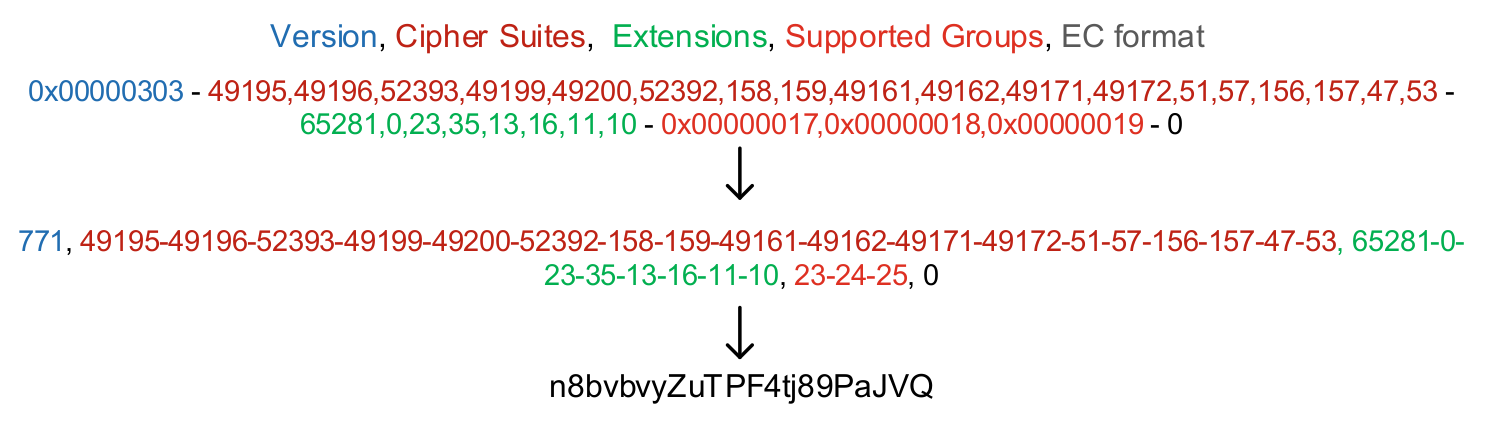
\includegraphics[width=0.99\linewidth]{ja3.png}
    \caption{Vytvoření JA3 otisku. Obrázek je převzatý~\cite{bib_matousek}.}
    \label{fig_ja3}
\end{figure}

Limitace tohoto řešení spočívá v~poměrně nízkém počtu možných otisků. Možností ustanovení TLS spojení není příliš velké. Porovnáváním pouze JA3 otisku pro danou aplikaci by nebylo dostatečné. Pravděpodobně pokud dvě aplikace využívají stejnou TLS knihovnu, jejich otisk bude stejný. Proto jako příznak pro rozpoznávání je třeba využít více informací, například SNI (\textit{Server Name Indication}).

%%%%%%%%%%%%%%%%%%%%%%%%%%%%%%%%%%%%%%%%%%%%%%%%%%%%%%%%%%%%%%%%%%%%%%%%%%%%%%%%

\newpage

%%%%%%%%%%%%%%%%%%%%%%%%%%%%%%%%%%%%%%%%%%%%%%%%%%%%%%%%%%%%%%%%%%%%%%%%%%%%%%%%

\section{Řešení}
\label{sec_solution}

\subsection{Vytvoření trénovací sady}

Pomocí nástroje pro vývojáře mobilních aplikací Android Studio\footnote{\url{https://developer.android.com/studio}} byl vytvořen virtuální mobilní telefon Google Pixel 4XL s~operačním systémem Android 11 a procesorovou architekturou x86.

Jelikož na takto vytvořený virtuální telefon není možné instalovat aplikace přes vestavěný klient Google Play, bylo nutné využít repozitáře třetích stran ApkMirror\footnote{\url{https://apkmirror.com}} nebo ApkPure\footnote{\url{https://apkpure.com}} a aplikace nainstalovat manuálně. Byl nainstalován následující seznam aplikací:

\begin{enumerate}
    \item \textit{Yr} v5.13.2,
    \item \textit{Settle Up: Group Expenses} v10.0.2030,
    \item \textit{Forest: Stay focused} v4.35.1,
    \item \textit{Forza Football: Live soccer scores} v5.1.13,
    \item \textit{Revolut} v7.43.1,
    \item \textit{GitHub} v1.7.4,
    \item \textit{Netflix} v7.97.1,
    \item \textit{Twitter} v8.88.0,
    \item \textit{YouTube} v16.12.34,
    \item \textit{Phoenix: The Bitcoin wallet from the future} v1.4.8.
\end{enumerate}

\begin{figure}[H]
    \centering
    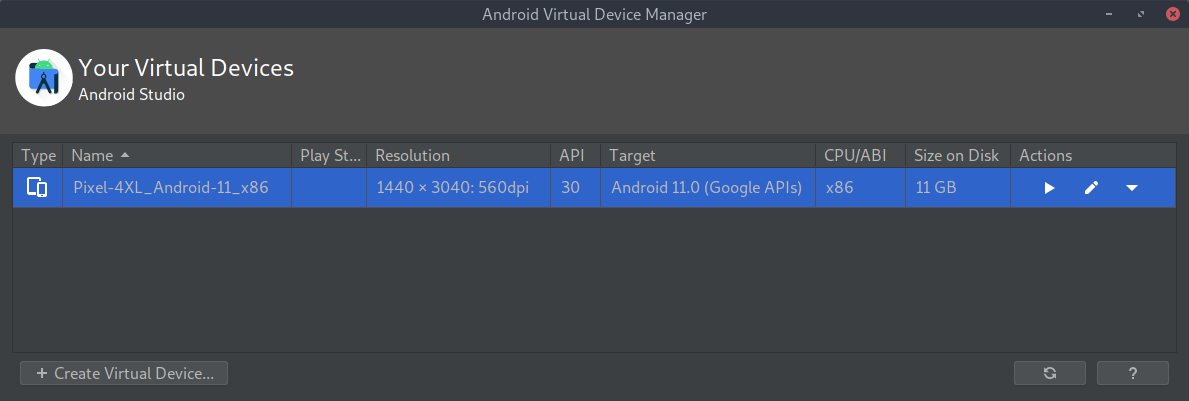
\includegraphics[width=0.99\linewidth]{android_virtual_device_manager.png}
    \caption{Program Android Virtual Device Manager pro správu virtuálních mobilních zařízení.}
    \label{fig_android_virtual_device_manager}
\end{figure}

\begin{center}
    \begin{lstlisting}[
        language=bash,
        caption={Spuštění virtuálního mobilního telefonu přes příkazový řádek na konkrétním portu.}
    ]
$ emulator -avd Pixel-4XL_Android-11_x86 -port 12345
\end{lstlisting}
\end{center}

\begin{figure}[H]
    \centering
    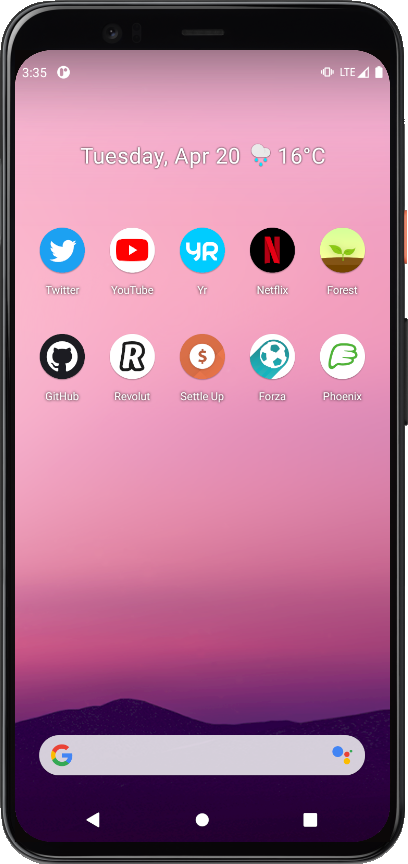
\includegraphics[width=0.25\linewidth]{google_pixel_4xl.png}
    \caption{Virtuální mobilní telefon Google Pixel 4XL s~operačním systémem Android 11 a nainstalovanými testovacími aplikacemi.}
    \label{fig_google_pixel_4xl}
\end{figure}

Pomocí klienta \texttt{adb} (\textit{Android Debug Bridge})\footnote{\url{https://developer.android.com/studio/command-line/adb}} je možné komunikovat s~virtuálním telefonem skrze příkazový řádek. Pro simulaci provozu jednotlivých aplikací byl použit nástroj \texttt{monkeyrunner}.\footnote{\url{https://developer.android.com/studio/test/monkeyrunner}} Ten lze přes \texttt{adb} spustit uvnitř telefonu. Programem Wireshark\footnote{\url{https://www.wireshark.org}} je možné poté odposlechnout síťový provoz a uložit jej jako \texttt{pcap} soubor.

\begin{center}
    \begin{lstlisting}[
    language=bash,
    caption={Spuštění 1000 náhodných událostí aplikace Phoenix.}
]
$ adb -s emulator-12345 shell monkey -p fr.acinq.phoenix.mainnet \ -v 1000
\end{lstlisting}
\end{center}

\begin{figure}[H]
    \centering
    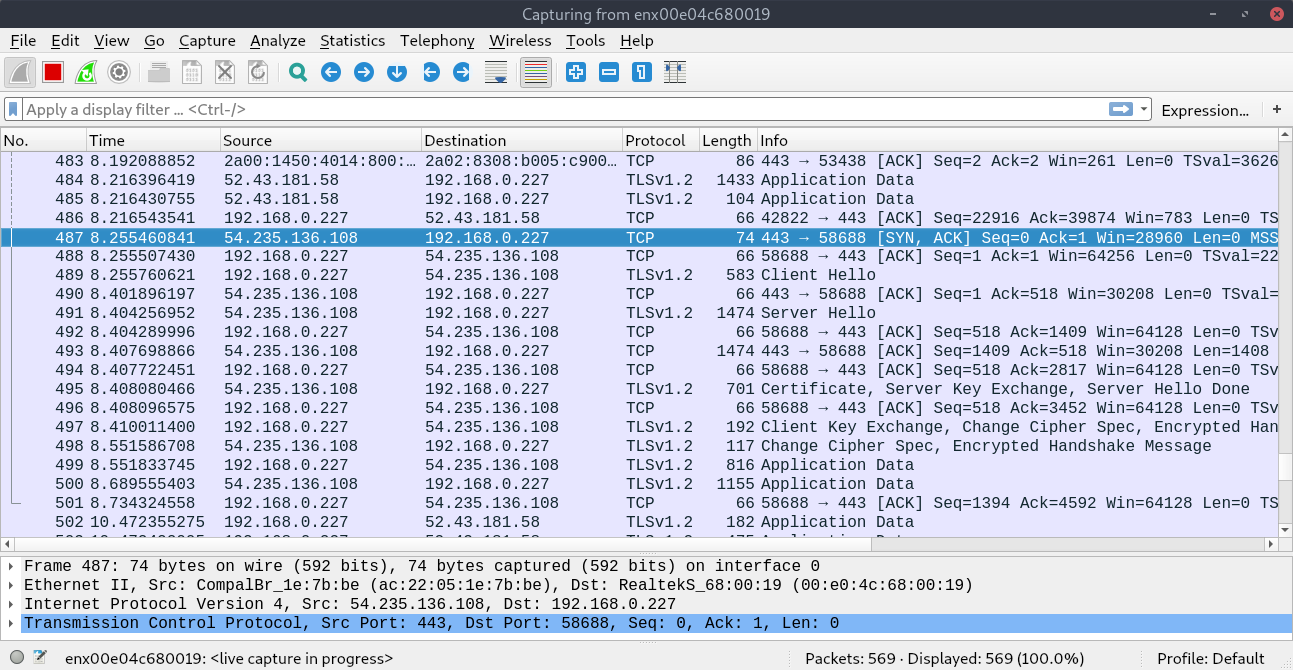
\includegraphics[width=0.99\linewidth]{wireshark.png}
    \caption{Zaznamenávání síťového provozu na virtuálním mobilním zařízení pomocí aplikace Wireshark.}
    \label{fig_wireshark}
\end{figure}

Tímto způsobem byla postupně zaznamenána komunikace každé z~vybraných aplikací. Celý postup byl opakován $6\times$. Celkově tedy bylo sesbíráno $60$ trénovacích \texttt{pcap} souborů. V~každém z~nich byla zaznamenána síťová komunikace během $1000$ náhodných událostí aplikace vyvolaných nástrojem \texttt{monkeyrunner}.

\subsection{Zpracování trénovací sady}

Pro zpracování \texttt{pcap} souborů byl využit jazyk Python a knihovna Pyshark\footnote{\url{https://github.com/KimiNewt/pyshark}}. Pyshark pouze zaobaluje Tshark\footnote{\url{https://www.wireshark.org/docs/man-pages/tshark.html}}, což je terminálová verze Wiresharku, do Python knihovny.

Zachycený provoz aplikací neobsahuje pouze komunikaci mezi telefonem a serverem aplikace samotné, ale také komunikace aplikací na pozadí a spojení s~reklamními a analytickými servery. Tyto spojení je nutné odfiltrovat. To bylo provedeno na základě sestavení \textit{whitelistu} podřetězců serverů (doménové jméno serveru musí obsahovat daný podřetězec), pro jednotlivé aplikace. Doménová jména serverů byla vypozorována z~komunikace jednotlivých aplikací.

\begin{center}
    \begin{lstlisting}[
        language=bash,
        caption={\textit{Whitelist} podřetězců komunikujících serverů pro jednotlivé aplikace.}
    ]
{
  "revolut": ["revolut"],
  "twitter": ["twitter", "twimg"],
  "phoenix": ["phoenix", "acinq"],
  "netflix": ["netflix", "nflxext"],
  "forza": ["forza"],
  "youtube": ["youtube", "ytimg", "redirector.googlevideo"],
  "yr": ["yr"],
  "forest": ["forest", "seekrtech"],
  "github": ["github"],
  "settleup": ["settleup", "settle-up"]
}
\end{lstlisting}
\end{center}

Z~veškeré zachycené komunikace byly vyfiltrovány TLS \textit{Client Hello} a TLS \textit{Server Hello} packety. Z~vybraných položek \textit{Handshake Version}, \textit{Cipher Suites}, \textit{Extensions}, \textit{Supported Groups} a \textit{Elliptic Curve Point Format} byl spočítán JA3 otisk pomocí hashovací funkce MD5. Takto byl spočítán otisk každého vyfiltrovaného packetu. Ze seznamů \textit{Cipher Suites}, \textit{Supported Groups} a \textit{Extensions} byly vymazány hodnoty GREASE (\textit{Generate Random Extensions And Sustain Extensibility}), \textit{renegotiation} a \textit{padding}. Které se objevují náhodně, případně jsou redundantní a do komunikace zavádějí nedeterminismus~\cite{bib_matousek}.

\begin{center}
    \begin{lstlisting}[
        language=bash,
        caption={Příklad výpočtu JA3 otisku z~TLS \textit{Client Hello} packetu.}
    ]
{
  "handshake_version": "771",
  "cipher_suites": "49195,49196,52393,49199,49200,52392,49171,49172,156,157,47,53",
  "extensions": "0,23,10,11,5,13",
  "supported_groups": "29,23,24"
  "ec_point_format": "0",
  "ja3_fingerprint": "2595ab65e691eb1d942c6094ff92c933"
}
\end{lstlisting}
\end{center}

Příznaky aplikací tvoří trojice následujícího formátu: JA3 otisk spočítáný z~TLS \textit{Client Hello}, JA3 otisk spočítaný z~TLS \textit{Server Hello} a SNI (\textit{Server Name Indication}), tedy doménové jménu serveru. Každé aplikaci připadá seznam příznaků. Všechny příznaky byly uloženy do souboru formátu \texttt{json}.

Odpovídající packety \textit{Client Hello} a \textit{Server Hello} byly propojeny na základě zdrojové/cílové IP adresy a zdrojového/cílového portu.

\begin{center}
    \begin{lstlisting}[
        language=bash,
        caption={Ukázka z~trénovací sady, příznaky aplikace Phoenix.}
    ]
{
  ...
  "phoenix": [
    {
      "client_ja3": "709c6b4bc7678a83ccc13a529103c873",
      "server_ja3": "77f87cbba1f72fcf7fbc308d9dcb561d",
      "sni": "phoenix.acinq.co"
    },
    {
      "client_ja3": "2595ab65e691eb1d942c6094ff92c933",
      "server_ja3": "b5c7a4c92e1f26c18a37bc9c1acd64b5",
      "sni": "acinq.co"
    },
    {
      "client_ja3": "cb533a60549e1e6021bd620b77ffce72",
      "server_ja3": "9758f7a0e1460a60e317ae2131b733a5",
      "sni": "electrum.acinq.co"
    }
  ],
  ...
}
\end{lstlisting}
\end{center}

%%%%%%%%%%%%%%%%%%%%%%%%%%%%%%%%%%%%%%%%%%%%%%%%%%%%%%%%%%%%%%%%%%%%%%%%%%%%%%%%

\newpage

%%%%%%%%%%%%%%%%%%%%%%%%%%%%%%%%%%%%%%%%%%%%%%%%%%%%%%%%%%%%%%%%%%%%%%%%%%%%%%%%

\section{Testování a vyhodnocení}
\label{sec_testing}

Pro otestování a vyhodnocení úspěšnosti detekce byla vytvořena testovací datová sada. Byly sesbírány $3$~\texttt{pcap} soubory s~komunikací každé z~natrénovaných aplikací a $10$~\texttt{pcap} souborů s~neznámou komunikací. Testovací datová sada byla vytvořena stejným způsobem jako trénovací.

Z~každého testovacího pcap souboru byly vyextrahovány všechny TLS \textit{Client Hello} a TLS \textit{Server Hello} packety. Byly spočítány jejich JA3 otisky a přes IP adresy a čísla portů byly propojeny. Takto byl sestaven příznak komunikace. Tímto způsobem byly z~konkrétního pcap souboru vyextrahovány všechny příznaky. Ty byly následně porovnávány se známými příznaky v~databázi. Aplikace která měla nejvíce shod byla vybrána.

Byly spočítány hodnoty TP (\textit{true positive}~--~skutečně pozitivní), FP (\textit{false positive}~--~falešně pozitivní), TN (\textit{true negative}~--~skutečně negativní) a FN (\textit{false negative}~--~falešně negativní) a z~nich metriky \textit{accuracy}, \textit{recall}, \textit{precision}. Kompletní výsledky testování jsou zaneseny v~tabulce~\ref{table_vysledky}.

\begin{itemize}
    \item $TP = 30$,\;\;$FP = 1$,\;\;$TN = 9$,\;\;$FN = 0$
    \item $Accuracy = \frac{TP + TN}{TP + TN + FP + FN} = 0,975$
    \item $Recall = \frac{TP}{TP + FN} = 1$
    \item $Precision = \frac{TP}{TP + FP} \approx 0,968$
\end{itemize}

\begin{table}[H]
    \centering
    \begin{tabular}{|c|c|c|}
        \hline
        Jméno souboru                       & Detekovaná aplikace & Výsledek   \\ \hhline{|=|=|=|}
        \path{forest-01.pcapng}             & Forest              & \checkmark \\ \hline
        \path{forest-02.pcapng}             & Forest              & \checkmark \\ \hline
        \path{forest-03.pcapng}             & Forest              & \checkmark \\ \hline
        \path{forza-01.pcapng}              & Forza               & \checkmark \\ \hline
        \path{forza-02.pcapng}              & Forza               & \checkmark \\ \hline
        \path{forza-03.pcapng}              & Forza               & \checkmark \\ \hline
        \path{github-01.pcapng}             & GitHub              & \checkmark \\ \hline
        \path{github-02.pcapng}             & GitHub              & \checkmark \\ \hline
        \path{github-03.pcapng}             & GitHub              & \checkmark \\ \hline
        \path{netflix-01.pcapng}            & Netflix             & \checkmark \\ \hline
        \path{netflix-02.pcapng}            & Netflix             & \checkmark \\ \hline
        \path{netflix-03.pcapng}            & Netflix             & \checkmark \\ \hline
        \path{phoenix-01.pcapng}            & Phoenix             & \checkmark \\ \hline
        \path{phoenix-02.pcapng}            & Phoenix             & \checkmark \\ \hline
        \path{phoenix-03.pcapng}            & Phoenix             & \checkmark \\ \hline
        \path{revolut-01.pcapng}            & Revolut             & \checkmark \\ \hline
        \path{revolut-02.pcapng}            & Revolut             & \checkmark \\ \hline
        \path{revolut-03.pcapng}            & Revolut             & \checkmark \\ \hline
        \path{settleup-01.pcapng}           & Settle Up            & \checkmark \\ \hline
        \path{settleup-02.pcapng}           & Settle Up           & \checkmark \\ \hline
        \path{settleup-03.pcapng}           & Settle Up            & \checkmark \\ \hline
        \path{twitter-01.pcapng}            & Twitter             & \checkmark \\ \hline
        \path{twitter-02.pcapng}            & Twitter             & \checkmark \\ \hline
        \path{twitter-03.pcapng}            & Twitter             & \checkmark \\ \hline
        \path{uknown-bitcoin.pcapng}        & $\times$            & \checkmark \\ \hline
        \path{uknown-gmail.pcapng}          & Twitter             & $\times$   \\ \hline
        \path{uknown-seznam.pcapng}         & $\times$            & \checkmark \\ \hline
        \path{unknown-damejidlo.pcapng}     & $\times$            & \checkmark \\ \hline
        \path{unknown-facebook.pcapng}      & $\times$            & \checkmark \\ \hline
        \path{unknown-google\_maps.pcapng}  & $\times$            & \checkmark \\ \hline
        \path{unknown-google\_photo.pcapng} & $\times$            & \checkmark \\ \hline
        \path{unknown-linkedin.pcapng}      & $\times$            & \checkmark \\ \hline
        \path{unknown-livesport.pcapng}     & $\times$            & \checkmark \\ \hline
        \path{unknown-stackoverflow.pcapng} & $\times$            & \checkmark \\ \hline
        \path{youtube-01.pcapng}            & YouTube             & \checkmark \\ \hline
        \path{youtube-02.pcapng}            & YouTube             & \checkmark \\ \hline
        \path{youtube-03.pcapng}            & YouTube             & \checkmark \\ \hline
        \path{yr-01.pcapng}                 & Yr                  & \checkmark \\ \hline
        \path{yr-02.pcapng}                 & Yr                  & \checkmark \\ \hline
        \path{yr-03.pcapng}                 & Yr                  & \checkmark \\ \hline
    \end{tabular}
    \caption{Tabulka s~kompletními výsledky testování úspěšnosti detekce.}
    \label{table_vysledky}
\end{table}

%%%%%%%%%%%%%%%%%%%%%%%%%%%%%%%%%%%%%%%%%%%%%%%%%%%%%%%%%%%%%%%%%%%%%%%%%%%%%%%%

\newpage

%%%%%%%%%%%%%%%%%%%%%%%%%%%%%%%%%%%%%%%%%%%%%%%%%%%%%%%%%%%%%%%%%%%%%%%%%%%%%%%%

\section{Závěr}
\label{sec_conclusion}

Natrénový detektor využívající kombinace JA3 otisku pro \textit{Client Hello} packet, JA3 otisku pro \textit{Server Hello} packet a doménového jména serveru dosáhl velmi dobrých výsledků na testovacích datech. Byla zaznamenána pouze jediná chyba, kdy provoz neznámé aplikace Gmail byl detekován jako aplikace Twitter.

Detekce neznámého TLS provozu pouze na základě JA3 otisků nemusí být příliš úspěšná~\cite{bib_matousek}. Tato úspěšnost může být zvýšena přídáním dalších informací do příznaků. Přidání doménového jména serveru, vyzkoušená v~tomto projektu, se ukázala jako velmi spolehlivá.

%%%%%%%%%%%%%%%%%%%%%%%%%%%%%%%%%%%%%%%%%%%%%%%%%%%%%%%%%%%%%%%%%%%%%%%%%%%%%%%%

\newpage

%%%%%%%%%%%%%%%%%%%%%%%%%%%%%%%%%%%%%%%%%%%%%%%%%%%%%%%%%%%%%%%%%%%%%%%%%%%%%%%%

\begin{thebibliography}{1}

    \bibitem{bib_matousek} Petr Matoušek, Ivana Burgetová, Ondřej Ryšavý, Malombe Victor: \textit{On Reliability of JA3 Hashes for Fingerprinting Mobile Applications}, 7. 2. 2021. Dostupné online na \url{https://rdcu.be/ci7mV}.

\end{thebibliography}

%%%%%%%%%%%%%%%%%%%%%%%%%%%%%%%%%%%%%%%%%%%%%%%%%%%%%%%%%%%%%%%%%%%%%%%%%%%%%%%%

\end{document}
